%%%%%%%%%%%%%%%%%%%%%%%%%%%%%%%%%%%%%%%%%%%%%%%%%%%%%%%%%%%%%%%%%
% Tese de Doutorado / Dept Fisica, CFM, UFSC                    %
% Andre@UFSC - 2014                                             %
%%%%%%%%%%%%%%%%%%%%%%%%%%%%%%%%%%%%%%%%%%%%%%%%%%%%%%%%%%%%%%%%%

%:::::::::::::::::::::::::::::::::::::::::::::::::::::::::::::::%
%                                                               %
%                          Capítulo 6                           %
%                                                               %
%:::::::::::::::::::::::::::::::::::::::::::::::::::::::::::::::%

%***************************************************************%
%                                                               %
%                       Efeitos da PSF                          %
%                                                               %
%***************************************************************%

\chapter{Efeitos da PSF}
\label{sec:psf}

%***************************************************************%
%                                                               %
%                       PSF do CALIFA                           %
%                                                               %
%***************************************************************%

\section{Medindo a PSF do CALIFA}

\TODO: O que é PSF. Modelos de Kolmogorov e Moffat.
Perfil de Moffat, dado pela equação
$$
I(r) = \frac{I_0}{\left(1 + (r / \alpha)^2\right)},
\alpha = \frac{\mathrm{FWHM}}{2\sqrt{2^{1/\beta} - 1}}.
$$

Para determinar as caraterísticas da PSF, idealmente é preciso observar um
objeto pontual brilhante, em várias regiões do campo de observação, e com as
mesmas condições atmosféricas que as observações. Raramente estas condições são
preenchidas, mesmo para fotometria CCD, que possuem campos muito grandes. Assim,
conhecer a PSF em instrumentos IFU não é uma tarefa trivial. Ainda há o fato de
que as imagens são reconstruídas através de técnicas de {\em dithering} (ver
Seção \ref{sec:ifs:instrumentacao}), e dependendo o algoritmo utilizado, a PSF
pode nem sequer ser analítica. Entretanto, é preciso de algum modo obter uma
aproximação da forma da PSF para poder modelar a morfologia de uma galáxia
(Capítulo \ref{sec:morph}), especialmente o seu bojo. Assim, o procedimento
descrito a seguir é mais um esforço para entender a PSF e poder realizar a
decomposição morfológica do que um estudo aprofundado sobre o tema.

Para o CALIFA, observar campos estelares para caracterizar a PSF significaria a
redução no número de galáxias na amostra final do {\em survey}. Dadas as
restrições de tempo de telescópio e de significância estatística da amostra,
além do fato de a PSF não ser fundamental para os casos científicos alvo do {\em
survey}, estas observações não foram realizadas. Porém, sendo um {\em survey}
espectroscópico, o CALIFA necessita de observações de ``velas padrão'' para
calibrar o fluxo das galáxias. Foram observadas 45 estrelas para este fim. Estas
estrelas foram obsevadas no centro no campo de observação do instrumento, com um
tempo de exposição muito menor do que o das galáxias (XX vs YY\fixme). Esta
amostra foi denominada ``estrelas de calibração''. Alternativamente, pode-se
procurar estrelas de campo que apareçam na frente das galáxias do {\em survey}.
Neste caso a vantagem é que as estrelas têm o mesmo tempo de exposição das
galáxias, e são observadas nas mesmas condições atmosféricas. Porém, não há
estrelas de campo em todos os cubos. Também, elas em geral são, por construção
do {\em survey}, fracas e se localizam na periferia do campo de observação.
Esta amostra foi denominada ``estrelas de campo''. A seguir são descritas duas
tentativas de caracterizar a PSF do CALIFA, utilizando ambas as amostras de
estrelas.

\begin{figure}
	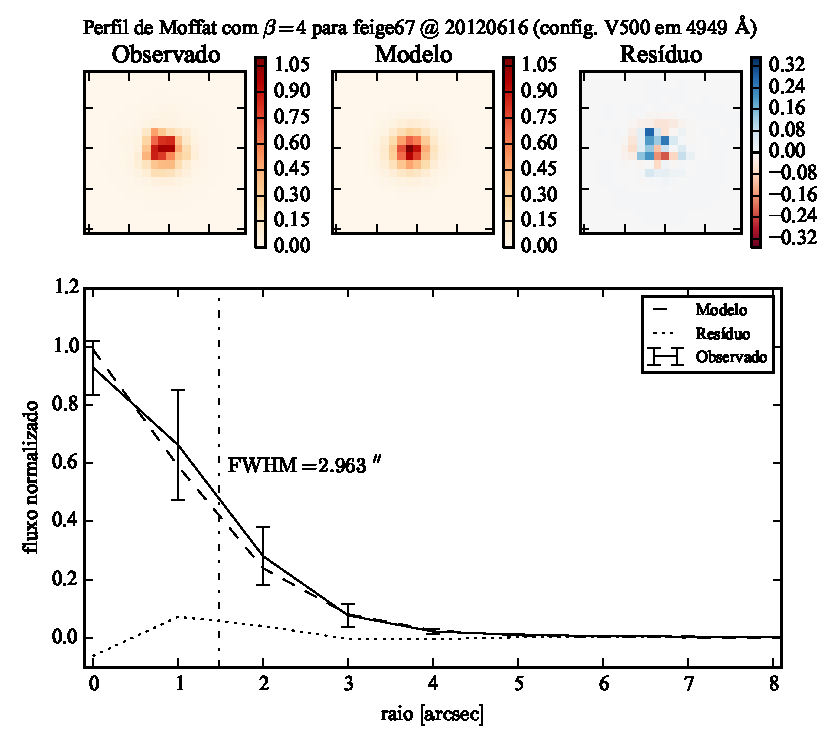
\includegraphics{figuras/PSFMoffatBeta4_exemplo}
	\caption[Exemplo de ajuste de PSF para estrela de calibração.]
	{Exemplo de ajuste de PSF para a estrela de calibração Feige67, observada em
	16/06/2012, com a cofiguração V500. O modelo ajustado foi um perfil de
	Moffat elipsoidal com $\beta=4$. Nos painéis superiores estão imagens do fluxo
	observado numa caixa de $400\,\angstrom$ centrada em $4949\,\angstrom$,
	do modelo ajustado e do resíduo do ajuste. No painel inferior mostra-se o
	perfil de brilho radial médio: observado (linha sólida, onde as barras de erro
	são $1\,\sigma$ da média), modelo (linha tracejada, e a linha traço-ponto marca
	a largura a meia altura $\mathrm{FWHM}=2,963\,"$) e resíduo (linha
	pontilhada).}
	\label{fig:PSFExemplo}
\end{figure}

O modelo utilizado foi um perfil de Moffat 2-d elipsoidal, com $\beta = 4$. Os
cubos foram combinados em caixas de $400\,\angstrom$ de largura, gerando 10
imagens de fluxo e incerteza para cada estrela. Estas imagens foram ajustadas
aos modelos através de um programa desenvolvido utilizando a biblioteca
PYTHON-IMFIT\footnote{PYTHON-IMFIT é uma biblioteca baseada no programa IMFIT de
\citet{Erwin2015}, a mesma utilizada no programa de decomposição morfológica,
ver Capítulo \ref{sec:morph}.}. O resultado do ajuste são os parâmetros do
perfil de Moffat e a estatística $\chi^2$ do melhor modelo. A Figura
\ref{fig:PSFExemplo} ilustra o ajuste feito para uma estrela de calibração, numa
faixa próxima a $5000\,\angstrom$.

\begin{figure}
	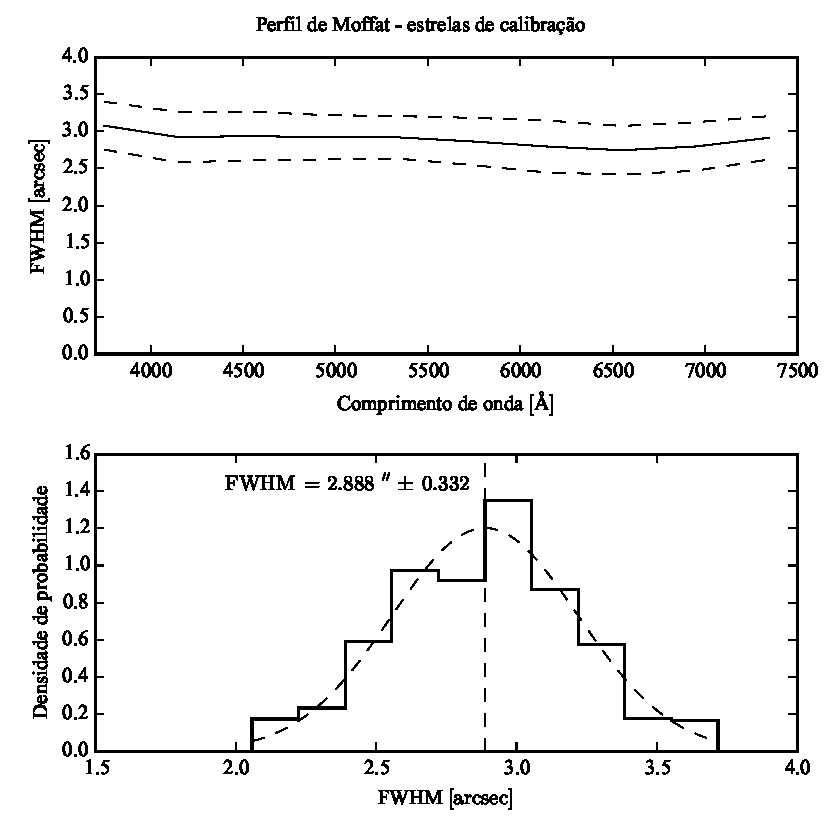
\includegraphics{figuras/PSFMoffatBeta4_calib}
	\caption[PSF do CALIFA -- estrelas de calibração.]
	{PSF do CALIFA modelada como um perfil de Moffat com $\beta=4$, utilizando 45
	estrelas de calibração. {\em Acima}: FWHM da PSF em função do comprimento de
	onda (caixas de $400\,\angstrom$). As linhas tracejadas indicam a distribuição
	em $1\ \sigma$. {\em Abaixo}: Histograma da FWHM da PSF, ponderado pela
	verossimilhança do modelo em todos os comprimento de onda de todas as estrelas,
	com $\mathrm{FWHM}=2,888\," \pm 0,332$.}
	\label{fig:PSFCalib}
\end{figure}

Este procedimento foi realizado para as 45 estrelas de calibração, e o resultado
pode ser visto na Figura \ref{fig:PSFCalib}. Praticamente não há dependência da
PSF com o comprimento de onda, como se pode verificar no painel superior da
figura. Na mesma figura, no painel inferior, mostra-se um histograma ponderado
pela verossimilhança ($\operatorname{e}^{-\chi^2/2}$) de todos os ajustes (todas
as estrelas em todas as caixas de comprimento de onda). Desta distribuição
obtém-se uma largura a meia altura\footnote{\TODO: FWHM footnte} média de
$\mathrm{FWHM}=2,888\," \pm 0,332$. A elipticidade média encontrada é de
$\epsilon=0,097 \pm 0,065$, ou seja, praticamente circular. A incerteza nos dois
casos representa o desvio padrão ($1\,\sigma$) da média ponderada. O mesmo vale
para todas as incertezas obtidas no resto desta seção.

\begin{figure}
	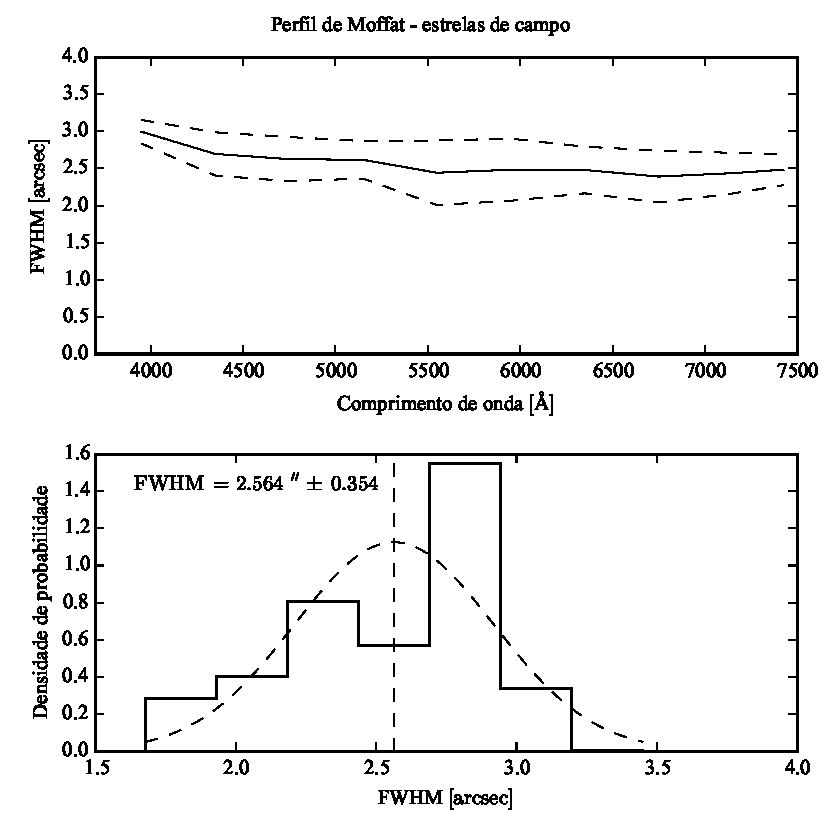
\includegraphics{figuras/PSFMoffatBeta4_field}
	\caption[PSF do CALIFA -- estrelas de campo.]
	{PSF do CALIFA modelada como um perfil de Moffat com $\beta=4$, utilizando 9
	estrelas de campo, na frente das galáxias observadas. {\em Acima}: FWHM da PSF
	em função do comprimento de onda (caixas de $400\,\angstrom$). As linhas
	tracejadas indicam a distribuição em $1\ \sigma$. {\em Abaixo}: Histograma da
	FWHM da PSF, ponderada pela verossimilhança do modelo em todos os comprimentos
	de onda de todas as estrelas, com $\mathrm{FWHM}=2,564\," \pm 0,354$.}
	\label{fig:PSFField}
\end{figure}

O mesmo procedimento foi realizado para 9 estrelas de campo, presentes nos cubos
de galáxias do {\em survey} e normalmente mascarados por não serem de interesse
no estudo do espectro das galáxias. Foram escolhidas galáxias com simetria axial
(elípticas e S0), com uma estrela razoavelmente brilhante na frente.
Dado um cubo de uma galáxia, recortou-se 7 {\em spaxels} ao redor da estrela,
gerando dois cubos: um da galáxia, com a estrela mascarada, e outro da estrela.
Neste ponto o cubo da estrela ainda está contaminado pela luz da galáxia. Então,
considerando que a galáxia tem simetria axial, calculou-se um perfil de brilho
radial médio da galáxia (ver Seção \ref{sec:pycasso:Pycasso}, Figura
\ref{fig:radprofIdade}), para cada comprimento de onda. Com este perfil, é
possível estimar quanto a galáxia está contribuindo para a luz de cada {\em
spaxel} do cubo da estrela, pois a distância de cada {\em spaxel} ao centro da
galáxia é conhecido. Criou-se assim um cubo de ``luz de fundo'' para a mesma
região que contém a estrela. Subtraindo o cubo de fundo do cubo da estrela,
obteve-se um cubo com apenas a luz proveniente da estrela.
Este cubo foi então analisado da mesma forma que os cubos de estrelas de
calibração, com os resultados mostrados na Figura \ref{fig:PSFField}. Da mesma
forma, não há dependência da FWHM da PSF com o comprimento de onda, com
$\mathrm{FWHM}=2,564\," \pm 0,354$ e elipticidade $\epsilon=0,093 \pm 0,059$.

Há uma diferença considerável no valor obtido para a FWHM da PSF nos dois casos,
embora eles estejam a cerca de $1\,\sigma$ de separação. Isto poderia indicar
uma diferença sistemática entre a PSF das estrelas de calibração e a PSF das
estrelas de campo. Todavia, observando atentamente o histograma de FWHM das
estrelas de campo (painel inferior da Figura \ref{fig:PSFField}), pode-se notar
que a distribuição possui um excesso próximo a $2,8\,"$. Isso parece indicar que
a FWHM da PSF das estrelas de campo é em geral maior do que o estimado pela
média ponderada, já que a distribuição se desvia de uma gaussiana. Isto, aliado
ao fato de que o tamanho da amostra de estrelas de calibração (45) é maior do
que o das estrelas de campo (9), fez com que se escolhesse a medida da primeira
amostra como a mais confiável. \TODO: Errar FWHM pra cima faz menos estragos?

Já com os valores de elipticidade ($\epsilon$) obtidos nos dois casos, os
semieixos maior e menor da FWHM estão dentro da faixa de $1\,\sigma$ um do
outro. E em ambos os casos, $\epsilon$ é muito próximo a zero, dentro da
incerteza. Levar a elipticidade em conta seria adicionar uma complexidade
desnecessária ao modelo de PSF.

Assim, a PSF adotada neste trabalho é um perfil de Moffat com simetria axial,
$\beta=4$ e $\mathrm{FWHM}=2,9\," \pm 0,3$. Este foi o mesmo procedimento para
fazer a caracterização da PSF publicada no DR2 do CALIFA
\citep{GarciaBenito2015}, mas com uma diferença. Naquele caso, modelou-se tanto
FWHM quanto $\beta$, obtendo-se $\mathrm{FWHM}=2,39\," \pm 0,26$ e
$\beta=1,73\," \pm 0,11$. \TODO: Por que escolhi fixar beta?

%***************************************************************%
%                                                               %
%                    PSF na decomposição                        %
%                                                               %
%***************************************************************%

\section{Efeito da PSF na decomposição morfológica}

\TODO: figuras dos modelos e ajustes.


% End of this chapter
